% !TeX root = main.tex
\lecture{20}{Thu 26 Mar 2026 13:00}{Fluid Dynamics}

\section{Fluid Dynamics}
Say we have no applied force, and the pressure at the liquid surface (for this weirdly shaped container) is $P_0$. What is the pressure $P$ at some depth $h$?

\begin{figure}[H]
    \centering
    
\includegraphics[width=0.35\textwidth]{figures/lec20-01.png}
     \caption{}
\end{figure}

\[
    P = P_0 + \rho g h
\]

If, and only if, the fluid has constant density $\rho$. If $\rho$ varied as a function of height, we'd need to start integrating.

What if we applied a force to the liquid at the top of the spout?
\begin{figure}[H]
    \centering
    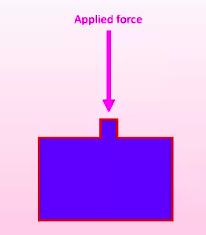
\includegraphics[width=0.35\textwidth]{figures/lec20-02.png}
     \caption{}
\end{figure}

Pressure in the liquid will increase, so the applied force to the walls of the container will increase. Pascal's law says that this increase in pressure is applied to every part of the fluid (and the walls of the enclosure) equally and undiminished.

\subsection{Example: Hydraulic Presses}
If we apply a force $F_1$ to a liquid in some very small cross-sectional area $a_1$, then the pressure this results in must be applied to all points in the liquid:
\[
    P = \frac{F_1}{a_1}
\]

Therefore, on the ``output'' of the press:

\[
    P = \frac{F_2}{a_2}
\]

If $a_2$ is much larger than $a_1$, the output force $F_2$ must be proportionally larger than the input force $F_1$ such that:
\[
    F_2 = \frac{F_1 a_2}{a_1}
\]

This effectively lets us magnify forces.

\subsection{Fluid in a Pipe}
In a steady state (a state with does not change with respect to time) the amount of water that passes a given point must also be constant with respect to time.
\begin{figure}[H]
    \centering
    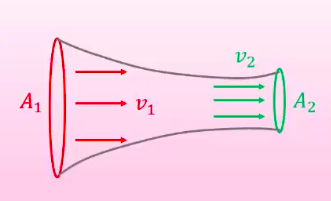
\includegraphics[width=0.75\textwidth]{figures/lec20-03.png}
     \caption{}
\end{figure}

For this to be a steady state, the amount of liquid passing both points must be the same (otherwise liquid would get stuck and build up). Therefore, we must see:
\[
    A_1 v_1 = A_2 v_2
\]

For $v_1 \neq v_2$, a force must be applied to the liquid to change velocity. This force comes from the neighbouring fluid molecules. 

Previously, we saw:
\[
    P = P_0 + \rho g h
\]

To account for the liquid now being non-stationary and having a velocity, we need to add a term accounting for pressure from kinetic energy:
\[
    P + \rho gh + \frac{1}{2} \rho v^2
\]

Here, $P$ is called static pressure, $\rho g h$ is called hydrostatic pressure and $\frac{1}{2} \rho v^2$ is called dynamic pressure. This full equation becomes useful in a context like this:

\begin{figure}[H]
    \centering
    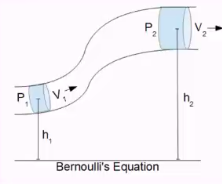
\includegraphics[width=0.35\textwidth]{figures/lec20-04.png}
     \caption{}
\end{figure}

\vspace{1cm}
\begin{center}
    \large \textbf{End of Module}
\end{center}
